\chapter{Développement}

Nous pouvons faire référence à des graphiques (très jolis au demeurant), comme
celui de la figure\vref{sin-x*sin-y}.
\lipsum[3-10]
\begin{figure}[ht]
  \centering
  \capstart
  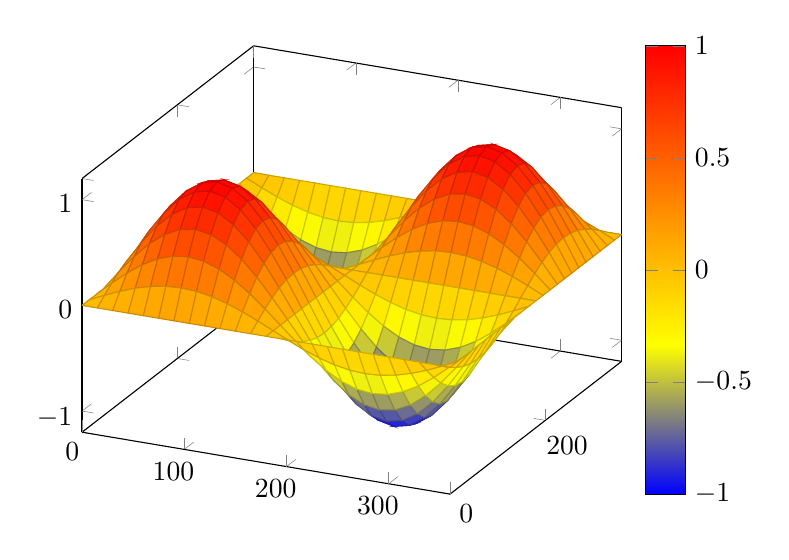
\begin{tikzpicture}
    \begin{axis}[colorbar]
      \addplot3[surf,domain=0:360]
      {sin(x)*sin(y)};
    \end{axis}
  \end{tikzpicture}
  \caption{Représentation graphique de la fonction $f:(x,y)\mapsto
    \sin x\times\sin y$}
  \label{sin-x*sin-y}
\end{figure}
